\documentclass[]{article}

%opening
\title{ Trabalho Final \\ Computação Evolucionária }
\author{Paulo CIrino Ribeiro Neto}


\usepackage[utf8]{inputenc}
\usepackage{float}
\usepackage{graphicx}

\begin{document}

\maketitle

\section{Introdução}

Problemas de localização de facilidades têm diversas aplicações em telecomunicações, transportes, orquestração de tarefas e distribuição. Uma importante maneira de medir a eficacia de uma localidade de uma facilidade e avaliando o decaimento da media (total) das distâncias em 
função do aumento da acessibilidade e eficiência da facilidade.

O problema da p-Mediana é um dos problemas mais conhecidos no âmbito de localização de facilidades, e ele aplica essa avaliação ao tentar minimizar a distancia total entre as demandas e um numero \textbf{p} de localidades selecionados, chamadas de medianas. O custo total da solução é a soma das distancias entre os pontos de demanda e as medianas.

Nesse trabalho o problema da p-Mediana capacitado e resolvido através de algoritmos genéticos, que se baseiam em heurísticas adaptativas que utilizam da ideia de avaliação do ``melhor adaptado''. Nesse trabalho é feita também uma
avaliação do impacto de diversos parâmetros nos resultados obtidos por meio de testes no dados fornecidos.

\section{Modelagem do Algorítimo Genético}
A modelagem do algorítimo genético se baseou no pseudo-código da figura abaixo e no material apresentado na Unidade III da disciplina.

\begin{figure}[H]
	\centering
	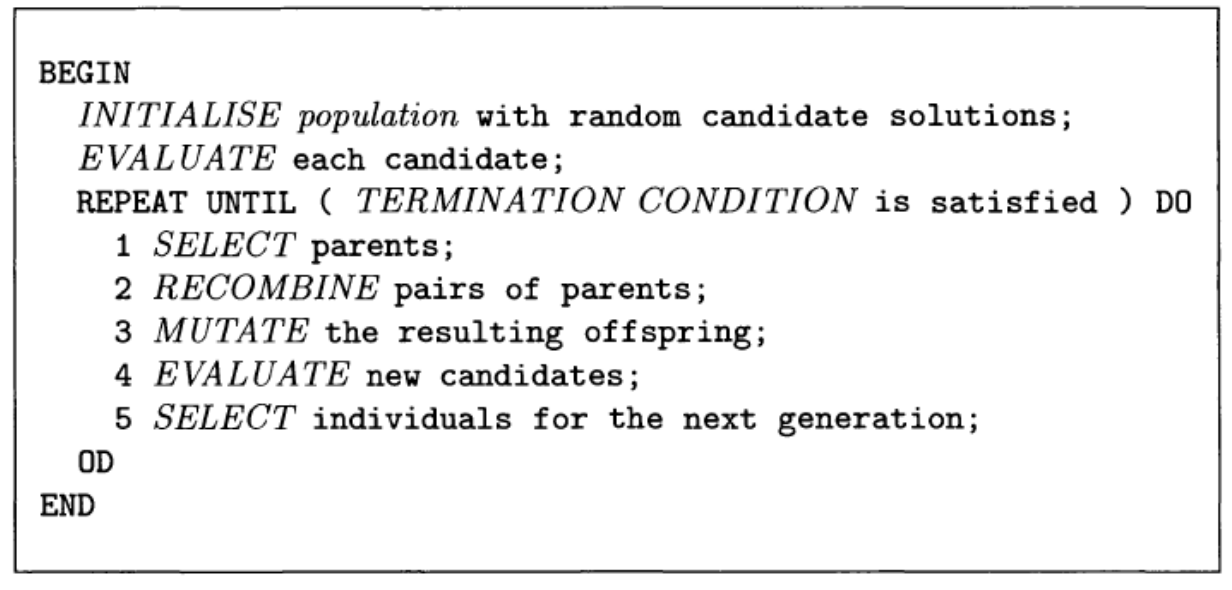
\includegraphics[scale = 0.5]{pics/GeneticAlgorithmPseudoCode.png}
	\caption{Pseudo Código - Algorítimo Genético}
	\label{fig:GeneticAlgorithmPseudoCode}
\end{figure}

\subsection{Representação do Indivíduo}
Cada solução candidata (indivíduo) possui exatamente \textbf{p} genes, onde \textbf{p} é o número de medianas do problema, e cada alelo de cada gene representa um dos \textbf{n} possíveis pontos de uma das facilidade. 

\subsection{Avaliação do \textit{Fitness}}
Dado que as medianas são selecionadas, o \textit{fitness} de uma solução candidata é o acumulado da soma das distâncias das facilidades à suas medianas mais próximas. 

Nesse caso em específico o indivíduo mais adaptado é o com menor soma acumulada.
\subsection{Seleção}
Algoritmos genéticos consistem de 4 operadores primários: 

\begin{itemize}
	\item [Reprodução] é o processo no qual características das soluções são passadas de uma geração para a outra. A solução candidata escolhida para reprodução é feita através de uma técnica de escolha aleatória de possíveis soluções ``pais'' e ao mesmo tempo enviesada para a escolha da maior \textit{fitness} por meio de de torneio;
	
	\item [\textit{CrossOver}] é o processo que combina soluções prévias para criação de novas soluções candidatas. Nesse caso, o \textit{crossover} é feito a partir de 2 soluções pais, com a recombinação aleatória dos seus genes para geração de 2 filhos;
	
	\item [Mutação] é o processo que garante variabilidade de genes entre as soluções. No caso desse trabalho, para cada de gene de cada solução existe uma probabilidade \textbf{P} de ele ser alterado para outro gene aleatório que não está presente na solução candidata.
	
	\item [Seleção de Sobreviventes] é onde inserimos um operador de elitismo, que garante que um número \textbf{e} das melhores soluções permanecerão entre as candidatas ao longo das execuções. As restantes \textbf{$n-e$} soluções são escolhidas aleatoriamente para frear a tomada da variabilidade genética pelas ``Super Soluções''.
\end{itemize}


\section{Implementação e Avaliação Experimental do Algorítimo}
O algorítimo foi implementado por meio de um \textit{script} em Matlab seguindo o pseudo-código apresentado na figura 1, onde cada uma das 
\section{Conclusões}

\section{Referências}

\end{document}
